\documentclass{beamer}
 
\usepackage[utf8]{inputenc}


\usetheme{Madrid}
\usecolortheme{default}
\usepackage{caption}
\usepackage{subcaption}
\usepackage{hhline}
\usepackage{graphicx}
\usepackage{physics}
\usepackage{amsmath}
\usepackage{amsfonts}
\usepackage{esint}
\usepackage{bbold}
\usepackage{mathtools}
\usepackage{dsfont}
\usepackage{amsthm}
\usepackage{bbm}
\usepackage{amssymb}
\theoremstyle{definition}
\newtheorem{defn}{Definition}[section]
\newtheorem{prop}{Properties}[section]
\newtheorem{rmk}{Remark}[section]
\newtheorem{exmp}{Example}[section]
\newtheorem{prob}{Problem}[section]
\newtheorem{proposition}{Proposition}
\newtheorem{thm}{Theorem}[section]
\newtheorem*{prob*}{Problem}
\newtheorem*{sln*}{Solution}
\usepackage{empheq}
\usepackage{tensor}

\newcommand{\lag}{\mathcal{L}}
\newcommand{\pOne}{\text{5p}_\text{1/2}}
\newcommand{\pThree}{\text{5p}_\text{3/2}}
\newcommand{\potassium}{^\text{39}\text{K}}
\newcommand{\R}{\mathbb{R}}
\newcommand{\lp}{\left(}
\newcommand{\rp}{\right)}
\newcommand{\lb}{\left[}
\newcommand{\rb}{\right]}
\newcommand{\lc}{\left\{}
\newcommand{\rc}{\right\}}
\newcommand{\p}{\partial}
\newcommand{\f}[2]{\frac{#1}{#2}}
\newcommand{\Vol}{\operatorname{Vol}}
\newcommand{\iprod}{\mathbin{\lrcorner}}
\newcommand{\al}{\alpha}
\newcommand{\be}{\beta}
\newcommand{\FT}{\mathcal{F}}
\newcommand{\LT}{\mathcal{L}}
\usepackage{hyperref}
\usepackage{tensor}
\usepackage{xcolor}
\hypersetup{
	colorlinks,
	linkcolor={black!50!black},
	citecolor={blue!50!black},
	urlcolor={blue!80!black}
}

% 3j symbol
\newcommand{\tj}[6]{ \begin{pmatrix}
		#1 & #2 & #3 \\
		#4 & #5 & #6 
\end{pmatrix}}
% 6j symbol
\newcommand{\Gj}[6]{ \begin{Bmatrix}
		#1 & #2 & #3 \\
		#4 & #5 & #6 
\end{Bmatrix}}

\setbeamerfont{title}{size=\large}

 
 
%Information to be included in the title page:
\title[\textcolor{white}{{Observation of vacuum-induced collective quantum beats}}]
{
	Observation of vacuum-induced collective quantum beats
}



\author[Bui] % (optional)
{Huan Q. Bui
	}

\institute[MIT] % (optional)
{
}
\date{ZGS, Jan 28, 2022}
 
%\logo{
\includegraphics[height=0.3cm]{colby.png}}
 
\begin{document}
 
\frame{\titlepage}



%%%%%%%%%%%%%%%%%%%%%%%%%%%%%%%%%%%%%%%%%%%%%%%%%%%%%%%%%%%%%%%%%%%%%%%%%

 
%\begin{frame}
%\frametitle{Layout}
%\tableofcontents
%\end{frame}

%%%%%%%%%%%%%%%%%%%%%%%%%%%%%%%%%%%%%%%%%%%%%%%%%%%%%%%%%%%%%%%%%%%%%%%%%




\begin{frame}
\textcolor{purple}{{Phys. Rev. Lett. \textbf{127}, 073604 – Published 13 August 2021}}
	\begin{figure}[!htb]
		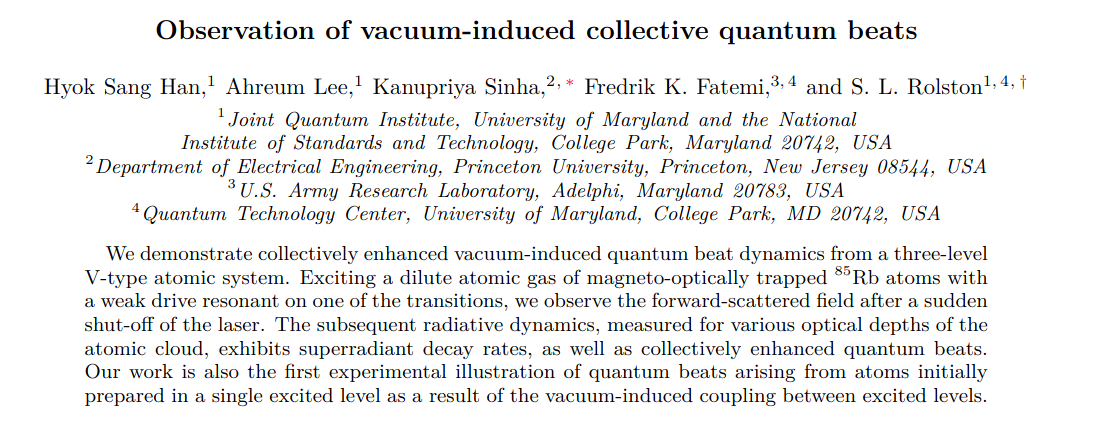
\includegraphics[width=1\textwidth]{abstract.png}
	\end{figure}
\end{frame}




\begin{frame}
\frametitle{Quantum beats}
\begin{itemize}
	\item Oscillatory behavior in the intensity of radiation emitted by atomic/molecular systems in a superposition of (excited) states
	
	\item Ex: quantum beats in the decay $\ket{5P_{3/2}}\to \ket{4S_{1/2}}$ in $^{39}$K
\end{itemize}




\begin{figure}[!htb]
	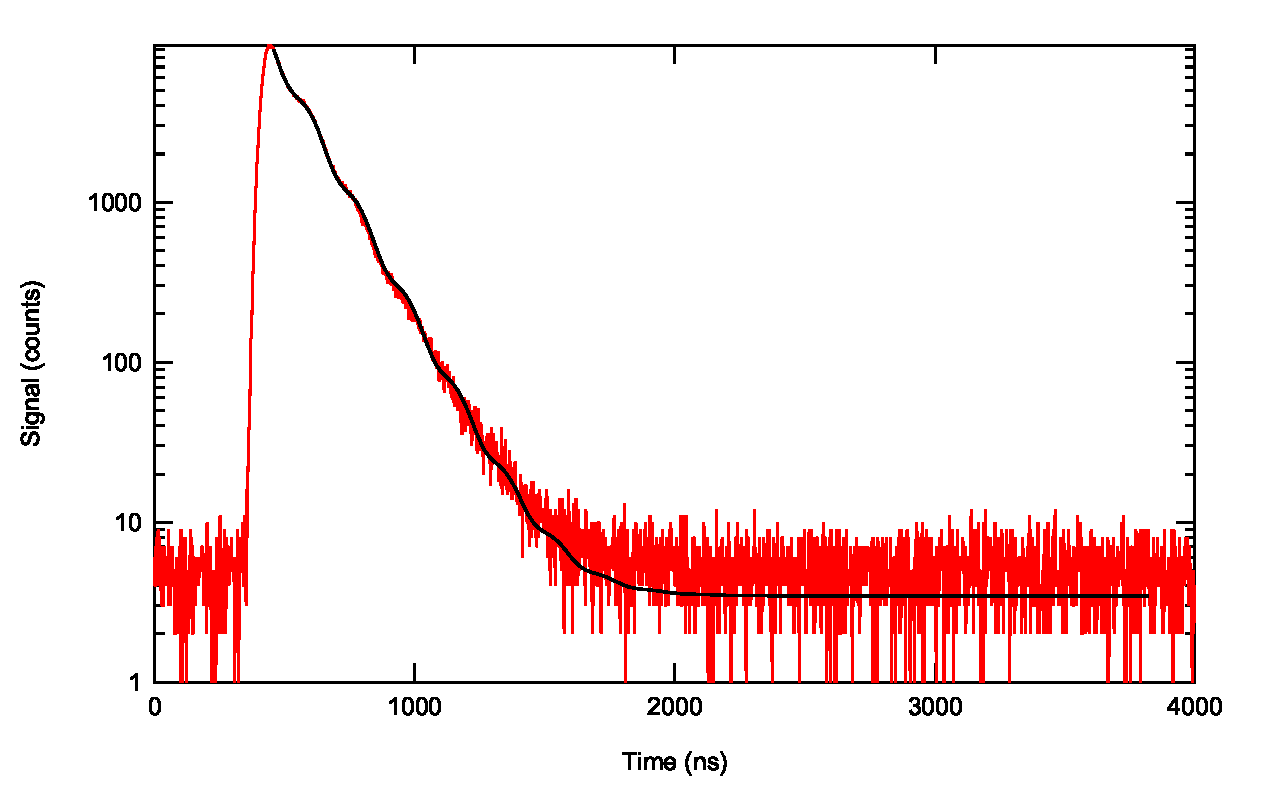
\includegraphics[width=0.6\textwidth]{big_beats_2.eps}
\end{figure}



\end{frame}




\begin{frame}
	Simplest case is the three-level system. Two types: $V$ and $\Lambda$.
	\begin{itemize}
		\item Semi-classical:
	\end{itemize}

\begin{figure}[!htb]
	\begin{subfigure}{0.4\textwidth}
		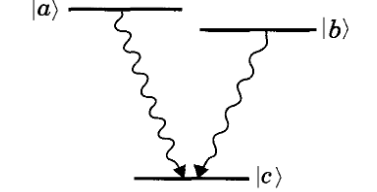
\includegraphics[width=\textwidth]{V.png}
	\end{subfigure}
	\begin{subfigure}{0.4\textwidth}
		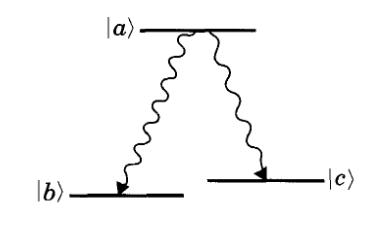
\includegraphics[width=\textwidth]{A.png}
	\end{subfigure}
\end{figure}
\begin{align*}
\ket{\psi(t)} = \al_a e^{-i \omega_a t}\ket{a} + \al_b e^{-i \omega_b t}\ket{b} + \al_c e^{-i \omega_c t}\ket{c}
\end{align*}
Each atom contains two oscillating dipoles:
\begin{align*}
e\bra{\psi(t)} r \ket{\psi(t)} = 
\begin{cases*}
\mathcal{P}_{ac} (\al_a^*\al_c) e^{i\nu_1 t} + \mathcal{P}_{bc}(\al_b^* \al_c) e^{i\nu_2 t} + c.c. \quad \text{if } V\\
\mathcal{P}_{ab} (\al_a^*\al_b) e^{i\nu_1 t} + \mathcal{P}_{ac}(\al_a^* \al_c) e^{i\nu_2 t} + c.c. \quad \text{if } \Lambda
\end{cases*}
\end{align*}
Radiated field:
\begin{align*}
E^{(+)} = \mathcal{E}_1 e^{-i\nu_1 t} + \mathcal{E}_2 e^{-i \nu_2 t} 
\implies \abs{E^{(+)}}^2 = \dots + \textcolor{purple}{[\mathcal{E}_1^*\mathcal{E}_2 e^{i(\nu_1 - \nu_2) t} + c.c.]}
\end{align*}
	
	
\end{frame}



\begin{frame}



Simplest case is the three-level system. Two types: $V$ and $\Lambda$.


\begin{itemize}
	\item QED:
\end{itemize}




\begin{figure}[!htb]
	\begin{subfigure}{0.4\textwidth}
		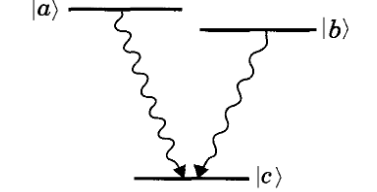
\includegraphics[width=\textwidth]{V.png}
	\end{subfigure}
	\begin{subfigure}{0.4\textwidth}
		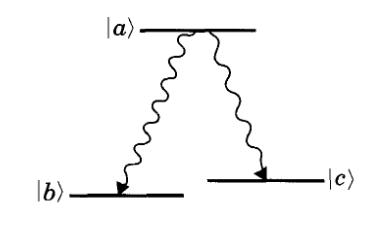
\includegraphics[width=\textwidth]{A.png}
	\end{subfigure}
\end{figure}


\begin{align*}
\ket{\psi_V(t)} &=  \sum_{i=a,b,c} \al_i \ket{i,0} + \al_1\ket{c,1_{\nu_1}} + \al_2 \ket{c,1_{\nu_2}}\\
\ket{\psi_\Lambda(t)} &=  \sum_{i=a,b,c} \al_i' \ket{i,0} + \al_1'\ket{b,1_{\nu_1}} + \al_2' \ket{c,1_{\nu_2}}
\end{align*}

\end{frame}


\begin{frame}
With
\begin{align*}
E^{(-)}_j(t) \sim a_j^\dagger e^{i\nu_j t} \quad \text{and} \quad E^{(+)}_j(t) \sim a_j e^{-i\nu_j t} 
\end{align*}
Beat note term:
\begin{equation*}
\bra{\psi_V(t)} E_1^{(-)}(t) E_2^{(+)}(t)  \ket{\psi_V(t)} \sim \bra{1_{\nu_1} 0_{\nu_2}} a_1^\dagger a_2 \ket{0_{\nu_1} 1_{\nu_2}} e^{i(\nu_1 - \nu_2)t} \underbrace{\braket{c}}_{1}
\end{equation*}

\begin{equation*}
\bra{\psi_\Lambda(t)} E_1^{(-)}(t) E_2^{(+)}(t)  \ket{\psi_\Lambda(t)} \sim \bra{1_{\nu_1} 0_{\nu_2}} a_1^\dagger a_2 \ket{0_{\nu_1} 1_{\nu_2}} e^{i(\nu_1 - \nu_2)t} \underbrace{\bra{c}\ket{b}}_{0}
\end{equation*}



\begin{itemize}
	\item Quantum beats can exist in $V$-type systems, but not in $\Lambda$-type
	
	
	\item This is not explained by semi-classical theory.
\end{itemize}

$\,$\\


\textcolor{purple}{\textbf{Textbooks: Quantum beats require a coherent superposition initially}}


\end{frame}



\begin{frame}
	\frametitle{"Observation of..." by Han et al.}
	
	Experimentally demonstrates 2 new aspects:
	\begin{itemize}
		\item \textbf{\textcolor{blue}{Vacuum-induced quantum beats:}} observed quantum beats without an initial superposition of excited levels
		
		
		\item \textbf{\textcolor{blue}{Collective effect:}} enhanced beat amplitudes and decay rates
	\end{itemize}
	
	
	
	
	
	
\end{frame}



\begin{frame}
	\frametitle{Experiment}
	
	\begin{figure}[!htb]
		\begin{subfigure}{0.55\textwidth}
			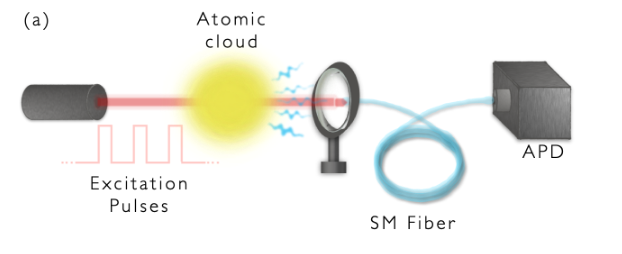
\includegraphics[width=\textwidth]{experiment.png}
		\end{subfigure}
		\begin{subfigure}{0.44\textwidth}
			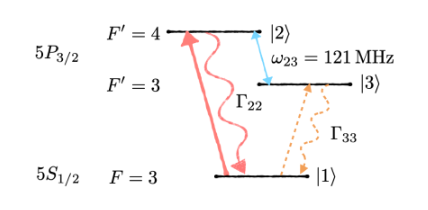
\includegraphics[width=\textwidth]{Rb85_levels.png}
		\end{subfigure}
	\end{figure}

\begin{itemize}
	\item $\sim 10^8$ $^{85}$Rb atoms in a MOT, $\rho \lambda^3 \ll 1$
	\item $V$-type system, well-separated. $\Gamma_{22} = 2\pi \cdot 6.1 $ MHz, $\Gamma_{33} = 5/9 \Gamma_{22}$
	\item $\Gamma_{23} \approx \sqrt{\Gamma_{22}\Gamma_{33}}$: 2nd order coupling between $\ket{2},\ket{3}$
	\item $v = 120 $ nm/\textmu s $\implies$ negligible to 780 nm over $1/\Gamma_{22}\approx 26$ ns
\end{itemize}
\end{frame}


\begin{frame}
	
	
	\begin{figure}[!htb]
		\begin{subfigure}{0.55\textwidth}
			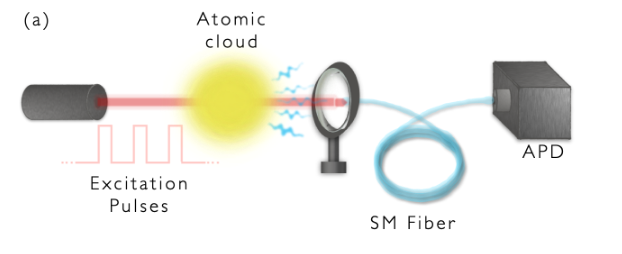
\includegraphics[width=\textwidth]{experiment.png}
		\end{subfigure}
		\begin{subfigure}{0.44\textwidth}
			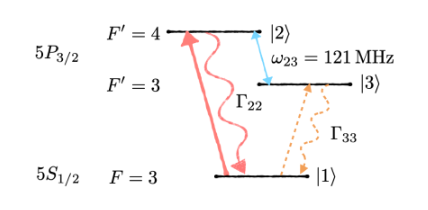
\includegraphics[width=\textwidth]{Rb85_levels.png}
		\end{subfigure}
	\end{figure}
	
\begin{itemize}
	\item Lin. pol. 780 nm light $(D_2)$ drives $\ket{1}\to \ket{2}$. 200 ns on, 800 ns off.  
	\item $> 30$ dB extinction ratio, 3.5 ns fall time (2 EOMs in series)
	\item $I_x \ll I_s = 3.9 \text{ mW/cm}^2 \implies$ single-excitation in $\ket{2}$
	\item Forward-scattered photons collected by SM fiber into APD 
	\item Histograms for $\sim$30 mins, new shot every 2 ms $\implies 2\times 10^8$ shots 
	
\end{itemize}
\end{frame}





\begin{frame}
	\frametitle{Data} 
	Raw histograms, taken at various $OD = -\ln T_s$
	\begin{figure}[!htb]
		\centering
		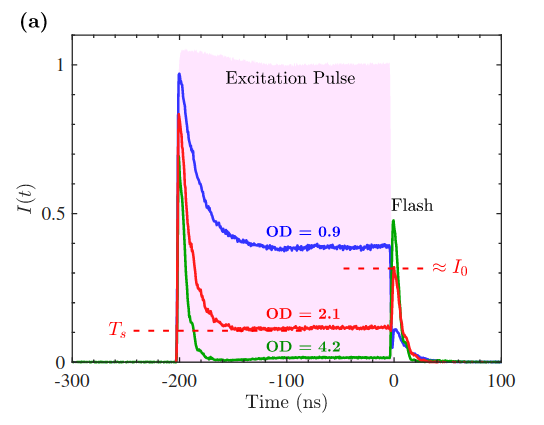
\includegraphics[width=0.5\textwidth]{data_full.png}
	\end{figure}
	\begin{itemize}
		\item $^{85}$Rb cloud is initially transparent
		\item Transmission decays to $T_s = e^{-OD}$, from destructive interference 
		\item "Flash" after driving field is switched off, amplitude $\propto OD$
	\end{itemize}

\end{frame}



\begin{frame}
	\begin{figure}[!htb]
		\centering
		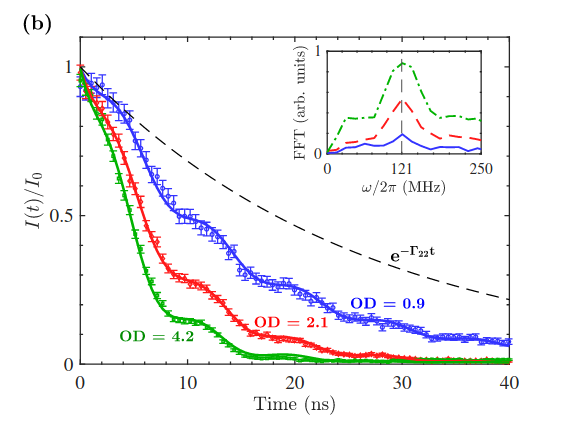
\includegraphics[width=0.5\textwidth]{data_zoom.png}
	\end{figure}
\begin{equation*}
I(t)/I_0 = e^{-\Gamma_{22}^{(N)}t} + I_b e^{-\Gamma_{\text{avg}}^{(N)}t} \sin(\omega_{23}t + \phi), \quad \begin{cases}
\textcolor{black}{\Gamma_{ij}^{(N)} = (1+ Nf) \Gamma_{ij}}\\
\textcolor{black}{\Gamma_\text{avg}^{(N)} = (\Gamma_{22}^{(N)} + \Gamma_{33}^{(N)})/2}
\end{cases}
\end{equation*}
\begin{itemize}
	\item From FFT, $f_\text{osc}\approx 121 $ MHz $= \omega_{23}/2\pi$, as expected
	\item Enhanced decay rates $\implies$ collective effect
	\item Fit parameters $I_b, \Gamma_{22}^{(N)}, \phi$ quantify collective effects
\end{itemize}


\end{frame}



\begin{frame}
	Collective effects:
	\begin{figure}[!htb]
		\centering
		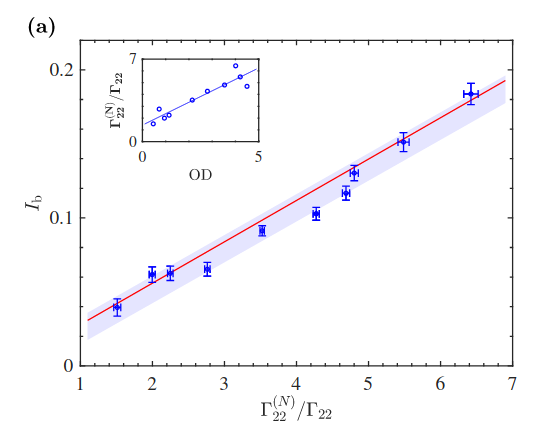
\includegraphics[width=0.5\textwidth]{data_Ib.png}
	\end{figure}
\begin{itemize}
	\item Enhanced decay rates: $\Gamma_{22}^{(N)}/\Gamma_{22} = 1.0(1) \cdot OD + 1.4(4)$
	
	\item Enhanced beat amplitude, in good agreement with
	\begin{align*}
	I_b = \f{\Gamma_{33}^{(N)}}{\omega_{23}} \approx \f{5}{9} \f{\Gamma_{22}^{(N)}}{\omega_{23}}
	\end{align*}
\end{itemize}
	
	


\end{frame}


\begin{frame}
	\frametitle{Model}
	\begin{align*}
	\mathcal{H}_\text{A} &= \sum_{m=1}^N \sum_{j=2,3} \hbar \omega_{j1}\, \hat\sigma_{m,j}^+ \hat\sigma_{m,j}^-  \\
	\mathcal{H}_\text{F} &= \sum_k \hbar \omega_k \, \hat a_k^\dagger \hat a_k\\
	\mathcal{H}_\text{AD} &= -\sum^N_{m=1}\sum_{j=2,3} \hbar \Omega^m_j \lp \hat \sigma_{m,j}^+ e^{-i \omega_D t} + \hat \sigma_{m,j}^- e^{i\omega_D t} \rp \\
	\mathcal{H}_\text{AF} &= -\sum^N_{m=1}\sum_{j=2,3} \sum_k \hbar g_{m,j}(\omega_k) \lp \hat \sigma_{m,j}^+ \hat a_k + \hat \sigma^-_{m,j} \hat a^\dagger_k\rp \quad \text{(RWA)}
	\end{align*}
\end{frame}


\begin{frame}
	\frametitle{Model: driven dynamics}
	
	Using experimental parameters to numerically solve for $\rho_A$
	\begin{itemize}
		\item $\rho_{33,s}\approx 0$
		\item $\rho_{22,s}\approx 10^{-10}$
		\item $\rho_{11,s}\approx 1$
		\item Only non-zero coherence: $\abs{\rho_{12}}^2 \approx 10^{-5}$
	\end{itemize}
$\implies$ Well within the single-excitation regime
\end{frame}


\begin{frame}
	\frametitle{Model: driven dynamics}
	Broad spectral component of turn-off may excite to $\ket{2},\ket{3}$
	\begin{figure}[!htb]
		\centering
		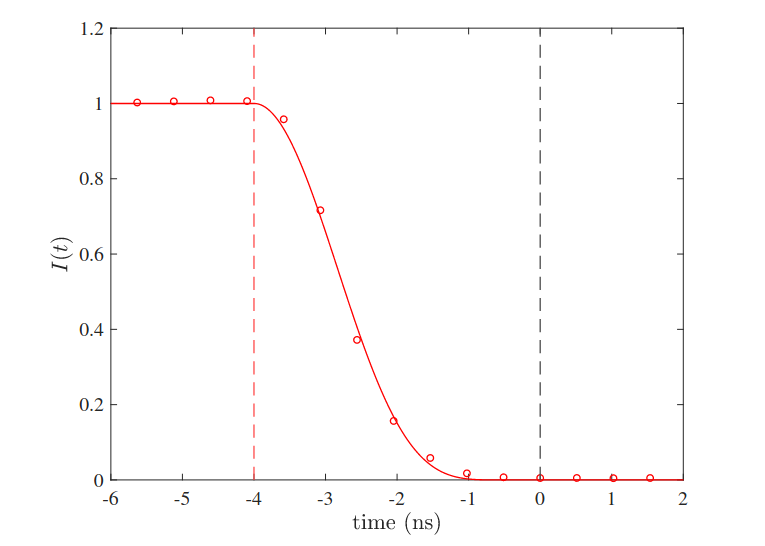
\includegraphics[width = 0.5\textwidth]{turn-off.png}
	\end{figure}
	$$\rho_{33}=\rho_{22} = \rho_{23} = 0, \rho_{11}=1, \rho_{12} = 10^{-5}, \rho_{13} \approx 10^{-6}$$
$\implies$ Laser turn-off produces no significant excitation \\
$\implies$ Wait 0.5 ns after turn-off to avoid residual drive \& transient effects.
\end{frame}




\begin{frame}
	\frametitle{Model: relaxation/quantum beat dynamics}
	Go to interaction representation w.r.t $\mathcal{H}_A + \mathcal{H}_F$ 
	\begin{align*}
	\widetilde{\mathcal{H}}_{AF} = -\sum^N_{m=1}\sum_{j=2,3} \sum_k \hbar g_j(\omega_k)\lp \hat \sigma_{m,j}^+ \hat a_k e^{i(\omega_{j1} - \omega_k) t} + \hat \sigma^-_{m,j} \hat a^\dagger_ke^{-i(\omega_{j1} - \omega_k) t}\rp
	\end{align*}
	Initially there is one excitation in $\ket{2}$ symmetrically:  
	\begin{align*}
	\ket{\psi(0)} &= \f{1}{\sqrt{N}} \sum^N_{m=1} \hat \sigma^+_{m,2} \ket{11\dots 1} \ket{\{0\}}\\
	\implies \ket{\psi(t)} &= \lp \sum^N_{m=1}\sum_{j=2,3} c_{m,j}(t)\hat \sigma_{m,j}^+ + \sum_k c_{\omega_k}(t)\hat a_k^\dagger \rp \ket{11\dots 1} \ket{\{0\}}
	\end{align*}
	Same IC, so $c_{m,j}(t) = c_{j}(t) \implies$ solve for $c_2(t), c_3(t)$ 
\end{frame}



\begin{frame}
	\frametitle{Model: relaxation/quantum beat dynamics}
	
	\begin{align*}
	c_2(t) &= \f{1}{\sqrt{N}} \lb e^{-\Gamma_{22}^{(N)} t/2} - \lp \f{\Gamma_{23}^{(N)}}{2\omega_{23}} \rp^2 \f{\delta^*}{\delta} e^{-\Gamma_{33}^{(N)}t/2} e^{i\omega_{23} t} \rb \\ 
	c_3(t) &= -\f{i\Gamma_{32}^{(N)}}{2\sqrt{N} \delta} \lb e^{-\Gamma_{22}^{(N)}t/2} e^{-i\omega_{23} t} - e^{-\Gamma_{33}^{(N)}t/2}  \rb
	\end{align*}
	
	\begin{itemize}
		\item Decay rate is $N$ times that of an individual atom (forward)
		\item Superradiance w.r.t both $\ket{2}$ (prep.) and $\ket{3}$ (vacuum-induced)
		\item Contribution of $\ket{3}$ creates quantum beats with frequency $\omega_{23}$
	\end{itemize}
\end{frame}





\begin{frame}
	\frametitle{Model: field intensity}
	
	Light intensity:
	\begin{align*}
	I(x,t) = \f{\epsilon_0 c}{2} \bra{\psi(t)} \hat E^+(x,t) \hat E(x,t) \ket{\psi(t)}
	\end{align*}
	E-field operator:
	\begin{align*}
	\hat E(x,t) = \int_\mathbb{R} dk\, E_k \hat a_k e^{ikx} e^{-i\omega_k t}
	\end{align*}
	Plugging in $\ket{\psi(t)}$ and eliminating $x$...
	\begin{align*}
	\f{I(t)}{I_0} &= e^{-\Gamma_{22}^{(N)}t} + \underbrace{\lp \Gamma_{33}^{(N)}/2\omega_{23} \rp^2}_{\ll 1} e^{-\Gamma_{33}^{(N)} t} + \underbrace{\lp\Gamma_{33}^{(N)}/\omega_{23} \rp}_{I_b}e^{-\Gamma_{\text{avg}}^{(N)}t} \sin(\omega_{23}t + \phi) \\
	&= e^{-(1+Nf)\Gamma_{22}t} + I_b e^{-\Gamma_{\text{avg}}^{(N)}t} \sin(\omega_{23}t + \phi)
	\end{align*}
\end{frame}



\begin{frame}
	
	\frametitle{Conclusion}
	\textbf{Summary:}
	
	\begin{itemize}
		\item Demonstrated collective quantum beats in spontaneous emission process \textcolor{blue}{without} initial superposition of excited states
		
		\item Observed 
		\begin{itemize}
			\item enhanced decay rates
			\item enhanced quantum beat amplitudes 
		\end{itemize}
		Good agreement with theoretical model and previous studies.

	\end{itemize}


	$\,$\\
	\textbf{Applications:}
	\begin{itemize}
		\item Tool in precision spectroscopy: enhancing signals
		
		\item Combined with waveguide optics to study interactions between distant atomic ensembles (e.g. ONF experiment at JQI)
	\end{itemize}
\end{frame}



\begin{frame}
	\frametitle{Extras: The phase term}
	Expect: $\phi = \arctan(\Gamma_{22}^{(N)}/\omega_{23})$
	\begin{figure}[!htb]
		\centering
		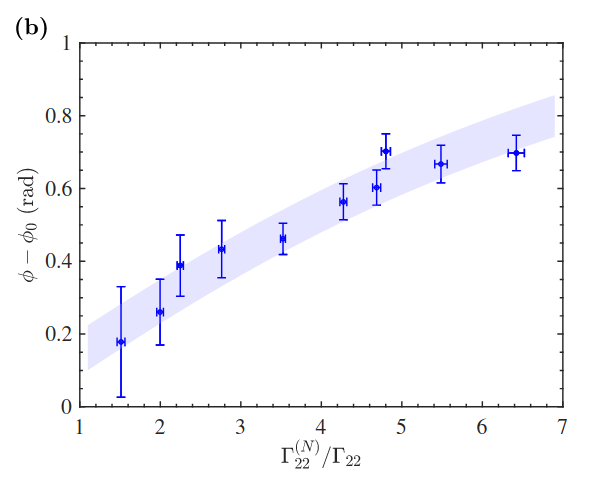
\includegraphics[width=0.5\textwidth]{phase}
	\end{figure}
	Fit to $
	\phi = \arctan(\eta \cdot \Gamma_{22}^{(N)}/\Gamma_{22}) + \phi_0$. Found $\eta \approx 3 \times \Gamma_{22}/\omega_{23}$ and $\phi_0 \neq 0$. 
	
	$\implies$ Possibly due to transience and non-equilibrium dynamics during switch off, causing OD-dependent phase delay not captured by the model. 
	
\end{frame}


\begin{frame}
\frametitle{References}
\begin{itemize}
	\item Scully, Marlan O., and M. Suhail Zubairy. "Quantum optics." (1999): 648-648.
	
	\item Han, Hyok Sang, et al. "Observation of vacuum-induced collective quantum beats." arXiv preprint arXiv:2102.11982 (2021).
\end{itemize}
\end{frame}



\end{document}